\documentclass[12pt]{report}

\usepackage[italian]{babel}
\usepackage{thesis}
\usepackage{parskip}
\usepackage{hyperref}
\usepackage{subfig}
\usepackage{graphicx}
\usepackage{siunitx}
\usepackage{booktabs}
\usepackage{array}
\usepackage{colortbl}

% Informazioni copertina
\university{Università degli Studi di Milano}
\unilogo{images/logos/unimi}
\faculty{Facoltà di Scienze e Tecnologie}
\department{Dipartimento di Informatica\\Giovanni Degli Antoni}
\cdl{Corso di Laurea Triennale in\\Informatica}

\title{Quantificazione e riduzione del sim-to-real gap in reti neurali addestrate per il riconoscimento di oggetti}

\author{Giovanni Novati}
\matricola{02108A}
\typeofthesis{Elaborato Finale}

\relatore{Prof. Nicola Basilico}
\correlatore{Prof. Michele Antonazzi}
\correlatore{Prof. Matteo Luperto}

\academicyear{2024} 

% Indice nell'indice
\tocintoctrue

\begin{document}

\makefrontpage

% Pagina di citazioni
{\raggedleft \large \sl
	
	\vspace{2cm}
	
	``Aut inveniam viam aut faciam''
	
	\bigskip
	
	\--- Annibale\\}

\beforepreface

% Creazione automatica dell'indice
\afterpreface

% CAPITOLO 1: Introduzione
\chapter{Introduzione}
\label{cap:introduzione}

\section{Robot di servizio}
\label{sec:robot_servizio}

I robot di servizio sono una tipologia di robot creata per assistere l'essere umano in ambienti antropocentrici, come abitazioni, uffici e ospedali, il tutto in maniera autonoma o semi-autonoma. L'obiettivo è semplificare la vita quotidiana delle persone, aumentando la sicurezza e la produttività.

Negli ultimi decenni questi robot sono stati adoperati in una varietà di scenari reali, come in ambienti domestici e industriali. Recentemente, queste tecnologie si sono sviluppate anche in settori come la sanità, andando ad assistere pazienti e caregiver~\cite{robotics10010047}; la logistica, dove svolgono compiti ripetitivi come la consegna di oggetti o il monitoraggio ambientale~\cite{fragapane2021405}; assistenza domiciliare, dove aiutano in attività quotidiane come la pulizia e assistenza alla persona.

Nonostante la diffusione di questi robot di servizio sia aumentata, il loro impiego in ambienti come case, scuole e uffici ha ancora diverse limitazioni. In un contesto industriale si ha un maggior grado di controllo e prevedibilità, caratteristiche non presenti in ambienti domestici che sono tipicamente non strutturati e dinamici. In ogni abitazione, aspetti come la planimetria e l'arredamento possono cambiare totalmente, oltre agli ostacoli presenti, siano essi mobili o fissi. A tutto questo si aggiungono anche i comportamenti imprevedibili di persone e animali, che possono interferire con le attività del robot~\cite{6301139}.

Un robot di servizio deve quindi riuscire a percepire e comprendere l'ambiente che lo circonda, così da poter svolgere compiti essenziali come la localizzazione, la pianificazione e la navigazione. Questo è possibile grazie a telecamere e sensori di profondità, che consentono di acquisire immagini e mappare lo spazio circostante, e a reti neurali che permettono di riconoscere e classificare oggetti. L'insieme di queste tecniche è comunemente chiamata \textit{robotic vision}.

\section{Problema della raccolta dati}
\label{sec:raccolta_dati}

L'addestramento di reti neurali è uno dei processi più importanti nella creazione di un sistema di robotic vision, e il suo corretto funzionamento dipende da vari fattori come la scelta del modello e dal processo di raccolta dei dati.

Per quanto riguarda la selezione del modello, a seconda delle attività che il robot deve svolgere si preferiscono determinate tipologie di modelli ad altre. Ad esempio, se si vogliono riconoscere oggetti in tempo reale si preferiscono reti neurali di tipo convoluzionale (CNN, Convolutional Neural Network)~\cite{oshea2015introductionconvolutionalneuralnetworks}, mentre se l'obiettivo è comprendere sequenze di azioni complesse, come nel caso dell'interazione con gli esseri umani, si opta in genere per reti neurali ricorrenti (RNN, Recurrent Neural Network)~\cite{ZHANG20209}. La sfida più grande non è però la scelta del modello, quanto la raccolta dei dati utilizzata per l'addestramento.

Raccogliere dati è da sempre un processo complesso in qualsiasi ambito, ma trova maggiori difficoltà in progetti di robotic vision. In questi casi, infatti, i dati vengono generalmente acquisiti facendo interagire robot con ambienti del mondo reale. Questo approccio ha però diverse limitazioni, dovute a fattori come il tempo e i costi che la raccolta comporta, oltre che per motivi inerenti la sicurezza di persone, animali e oggetti presenti nell'ambiente. A questi elementi si aggiunge anche il fattore riproducibilità, che viene meno quando si hanno variazioni nell'hardware utilizzato o negli ambienti considerati, e che può condurre a risultati differenti.

\section{Addestramento con dati simulati}
\label{sec:addestramento_dati_simulati}

Una possibile soluzione a questi problemi è l'utilizzo di ambienti simulati per la raccolta di dati. Questo permette infatti di ottenere dati a basso costo, in quanto non è necessario impegnare veri ambienti e robot, in tempi più brevi, grazie al fatto che le simulazioni possono essere velocizzate o parallelizzate, e senza i possibili rischi che una reale interazione con l'ambiente comporta.

Un simulatore consente inoltre di conoscere in anticipo e progettare gli scenari in cui un robot andrà ad interagire, andando a regolare vari parametri così da controllarne ogni singolo aspetto. Questo garantisce che l'ambiente non vari ed evolva nel tempo, a meno che non sia stato appositamente programmato per farlo.

Questo approccio permette di risolvere molti problemi, ma ne introduce di nuovi. La simulazione è infatti solo un'approssimazione della realtà, e non è possibile replicare fedelmente tutti i fenomeni e le caratteristiche del mondo reale. I motivi per i quale queste tipologie di ambienti differiscono sono principalmente due: il fotorealismo e l'interazione fisica.

Per fotorealismo si intende la capacità del simulatore di riprodurre in maniera visivamente accurata ambienti reali, in modo dettagliato e credibile. Tuttavia, risulta difficile replicare fenomeni come l'illuminazione, le riflessioni e texture di superfici. Questa mancanza di dettaglii ha un grande impatto sulla qualità dei dati raccolti per l'addestramento, con una conseguente mancanza di generalizzazione nel mondo reale da parte del modello.

L'interazione fisica si riferisce invece all'abilità del simulatore di riuscire a replicare le leggi della fisica in maniera realistica; questo comprende ad esempio il movimento e l'interazione tra oggetti.

In questi ultimi anni sono stati sviluppati diversi nuovi simulatori~\cite{kolve2022ai2thorinteractive3denvironment}~\cite{NEURIPS2021_021bbc7e}~\cite{urakami2022doorgymscalabledooropening}~\cite{1389727}, ognuno specializzato per specifici casi d'uso, e tutti si concentrano pervalentemente su uno dei due aspetti sopra citati.

Reti neurali addestrate con dati provenienti da simulatori e testati negli stessi ambienti simulati, otterranno risultati eccellenti. Sapranno infatti individuare e riconoscere correttamente gli oggetti presenti, in quanto il dominio dei dati utilizzato per l'addestramento e quello usato per il testing è lo stesso. Invece, l'adozione di reti naurali addestrare con dati sintetici in ambienti reali, avranno performance scadenti, non riuscendo neanche a riconoscere le categorie di oggetti più comuni presenti nel mondo reale~\cite{8793591}. Questo problema è noto come \textit{sim-to-real gap}, letteralmente 'divario tra simulazione e realtà', e rappresenta la differenza di prestazioni tra un modello addestrato in un ambiente simulato, e le performance nel mondo reale.

Una soluzione che permette di mitigare questo problema è l'adozione di una tecnica chiamata domain randomization , che permette di variare caratteristiche ed oggetti presenti nell'ambiente simulato (posizione e tipi di oggetti, illuminazione, texture). Questo permette di rendere il modello più robusto, permettendogli di operare meglio in contesti reali.

% CAPITOLO 2: Stato dell'Arte
\chapter{Stato dell'arte}
\label{chap:stato_arte}

Il sim-to-real gap è uno dei principali problemi nel campo della robitic vision, in quanto la complessità degli ambienti reali va oltre quello che è possibile rappresentare attraverso una simulazione. In questi ultimi anni la comunità scientifica si è interessata a questo problema, e ha provato a proporre delle soluzioni.

\section{Domain adaptation}
\label{sec:adaptation}

Quella del domain adaptation è una delle strategie più utilizzate per cercare di ridurre il sim-to-real gap, in quanto si cercano di ridurre le differenze tra l'ambiente simulato e quello reale. Questa tecnica si basa sul trasformare i dati provenienti dal simulatore, in modo da farli assomigliare il più possibile a quelli raccolti nel mondo reale. Il processo di trasformazione dei dati comprende l'utilizzo di tecnologie come le reti generative avversarie (GAN, Generative Adversarial Network)~\cite{10.1145/3422622}, che utilizzano in genere due diverse reti neurali per migliorare la qualità dei dati simulati. Una rete crea nuove immagini, il più simili possibili a quelle reali, mentre l'altra valuta la bontà delle immagini generate, che devono essere il più realistiche possibili. Questo approccio si è rivelato particolarmente efficace e ha permesso di migliorare le performance di generalizzazione nei modelli di robotic vision~\cite{Shrivastava_2017_CVPR}.

Ad esempio, un'immagine presa da un ambiente simulato, con texture uniformi e un'illuminazione predefinita, può essere trasformata in una più fotorealistica variando la luce, aggiungendo riflessioni e creando imperfezioni sulla superficie di oggetti. In pratica si cerca di aggiungere caratteristiche presenti nel mondo reale a dati campionati da simulatori, in modo da ridurre la differenza tra quello che è il dominio della simulazione e quello della realtà.

\section{Data augmentation}
\label{sec:augmentation}

Un ulteriore approccio per ridurre il sim-to-real gap è quello di augmentare i dati reali disponibili durante il training. La data augmentation è una tecnica molto diffusa nel campo della robotic vision, e consiste nell'applicare trasformazioni a dataset reali con l'obiettivo di aumentare sia il numero di dati disponibili, che l'eterogeneità dei dati stessi~\cite{Shorten2019}. Queste trasformazioni possono comprendere rotazioni, ridimensionamenti, traslazioni, e l'applicazione di filtri che possano simulare condizioni ambientali come nebbia, riflessi e occlusione ambientale. La data augmentation permette sia di aumentare la dimensione di dataset senza la necessità di campionare nuovi dati, sia consente ai modelli di generalizzare meglio a variazioni presenti nel mondo reale. Consideriamo ad esempio un robot che deve riuscire a riconoscere e classificare oggetti in ambienti con un'illuminazione dinamica; applicare filtri per simulare differenti condizioni di luce può migliorare significativamente le sue abilità di generalizzazione~\cite{NEURIPS2021_fb4c4860}. Inoltre, la data augmentation può essere usata in presenza di dataset sbilanciati, nei quali alcune classi sono sottorappresentate rispetto ad altre. Attraverso una serie di trasformazioni è infatti possibile aumentare il numero di dati appartenenti alle classi meno presenti, migliorando di conseguenta le capacità del modello nel riconoscerle.

Un'altro esempio nel quale questa tecnica può tornare utile, è nel caso si vengano a creare dipendenze da caretteristiche non rilevanti (bias). Ad esempio, se un modello tende ad associare la presenza di uno specifico sfondo a quella di un particolare oggetto, può essere conveniente effettuare trasformazioni andando a modificare o rimuovere lo sfondo, in modo da rendere indipendente la presenza di un oggetto da quella di un'altro.

Un esempio di bias è ben descritto nell'articolo~\cite{diagnostics12010040}, relativo ad un modello addestrato a riconoscere melanomi da tessuti sani. La rete neurale è stata addestrata a partire da un dataset contenente foto raffiguranti tumori maligni e tessuti epiteliali sani. Sebbene i risultati di validazione fossero inizialmente promettenti, si è scoperto che il modello non aveva realmente imparato a riconoscere la presenza di melanomi. Piuttosto, basava le sue previsioni su correlazioni spurie presenti nei dati. Nelle immagini raffiguranti tessuti sani erano sempre presenti artefatti come righelli e altri strumenti di calibrazione, che erano invece assenti in quelle rappresentanti tumori maligni. Come conseguenza, questi dati hanno portato il modello a trovare delle \textit{scorciatoie} (shortcut learning), utilizzando la presenza di questi artefatti come principale regola per classificare le immagini.

\section{Domain randomization}
\label{sec:randomization}

Invece che addestrare un modello su una singola scena simulata creata manualmente, la domain randomization permette di randomizzare gli elementi come oggetti, luce, texture ed eventuale rumore in maniera automatica all'interno di uno stesso ambiente. Questo consente al modello di imparare molteplici dispozizioni di oggetti e caratteristiche, migliorandone così le capacità di generalizzazione. Con questo approccio si cercano quindi di ricreare le condizioni che caratterizzano un normale ambiente domestico; a distanza di pochi giorni è raro che vengano introdotti o rimossi degli oggetti, mentre è molto più probabile che oggetti già presenti vengano spostati. Questo comporta una diversa disposizione degli oggetti, con una conseguente differenza nell'illuminazione della stanza, nei riflessi, e possibilmente anche nei colori. Se il modello non è abbastanza robusto a questo tipo di cambiamenti, potrebbe non riuscire a generalizzare correttamente.

Questa tecnica~\cite{8202133} è particolarmente efficace nell'addestrare reti neurali profonde (DNN, Deep Neural Netework) per compiti come l'identificazione e la manipolazione di oggetti. Ha infatti permesso di addestrare un modello utilizzando solo immagini simulate, riuscendo poi a localizzare in maniera accurata oggetti in ambienti reali, senza necessitare di ulteriori dati provenienti dal mondo reale.

La domain randomization permette quindi di generare grandi dataset di addestramento col minimo sforzo da parte di un operatore umano, e di ottenere modelli robusti senza la necessità di effettuare fine tuning con dati reali.

% CAPITOLO 3: Soluzione proposta
\chapter{Soluzione proposta}
\label{chap:soluzione}

Abbiamo visto che per addestrare un modello di deep learning è necessario un gran numero di dati, e che la campionatura di quest'ultimi nel mondo reale comporta spesso tempi e costi troppo elevati; si è quindi deciso di utilizzare un simulatore per la raccolta dei dati. Il risvolto negativo è però il divario tra simulazione e realtà, in quanto il modello dovrà essere utilizzato in ambienti reali. Bisogna quindi cercare di mitigare il problema del sim-to-real gap.

\section{Idea}
\label{chap:idea}

Come discusso nel \hyperref[chap:stato_arte]{Capitolo \ref{chap:stato_arte}}, gli approcci più utilizzati in letteratura per affrontare questo problema consistono nel modificare i dati simulati così da renderli il più possibile simili a quelli reali. Nel presente lavoro, tuttavia, abbiamo scelto di risolvere il problema inverso, ovvero trasformare i dati reali per renderli il più simili possibile a quelli generati dall'ambiente simulato. In questo contesto, non ci concentriamo più sul sim-to-real gap, ma sull'opposto, ovvero sul problema del \textit{real-to-sim gap}~\cite{8620258}~\cite{Prakash_2021_ICCV}.

Per fare ciò dobbiamo innanzitutto stabilire il nostro obiettivo finale, ovvero capire quali caratteristiche (\textit{feature}) il nostro modello deve riuscire a rilevare all'interno dell'ambiente. Nel nostro caso vogliamo riuscire a riconoscere determinate classi di oggetti e individuarne i contorni precisi; ci interessa quindi effettuare un task di segmentazione.

La segmentazione può essere suddivisa in due categorie: semantica e d'istanza. La prima consiste nell'assegnare a ciascun pixel di un'immagine un valore che indica a quale classe appartiene l'oggetto rappresentato da quel pixel. La seconda invece, non solo associa un valore di classe a ciascun pixel, ma identifica in maniera univoca ogni oggetto, consentendo di distinguere tra oggetti appartenenti alla stessa classe. Un esempio di segmentazione semantica e segmentazione d'istanza è illustrato nella \hyperref[fig:segmentazione]{Figura \ref{fig:segmentazione}}.

In questo lavoro si è deciso di adottare la segmentazione semantica, in quanto ci consente di semplificare il lavoro del modello, e di conseguenza ridurne la complessità. Questo è l'ideale nel campo della robotica mobile, in quanto porta a un minor carico computazionale e di conseguenza ad una maggiore autonomia.

\begin{figure}[t]
	\centering
	\subfloat[]{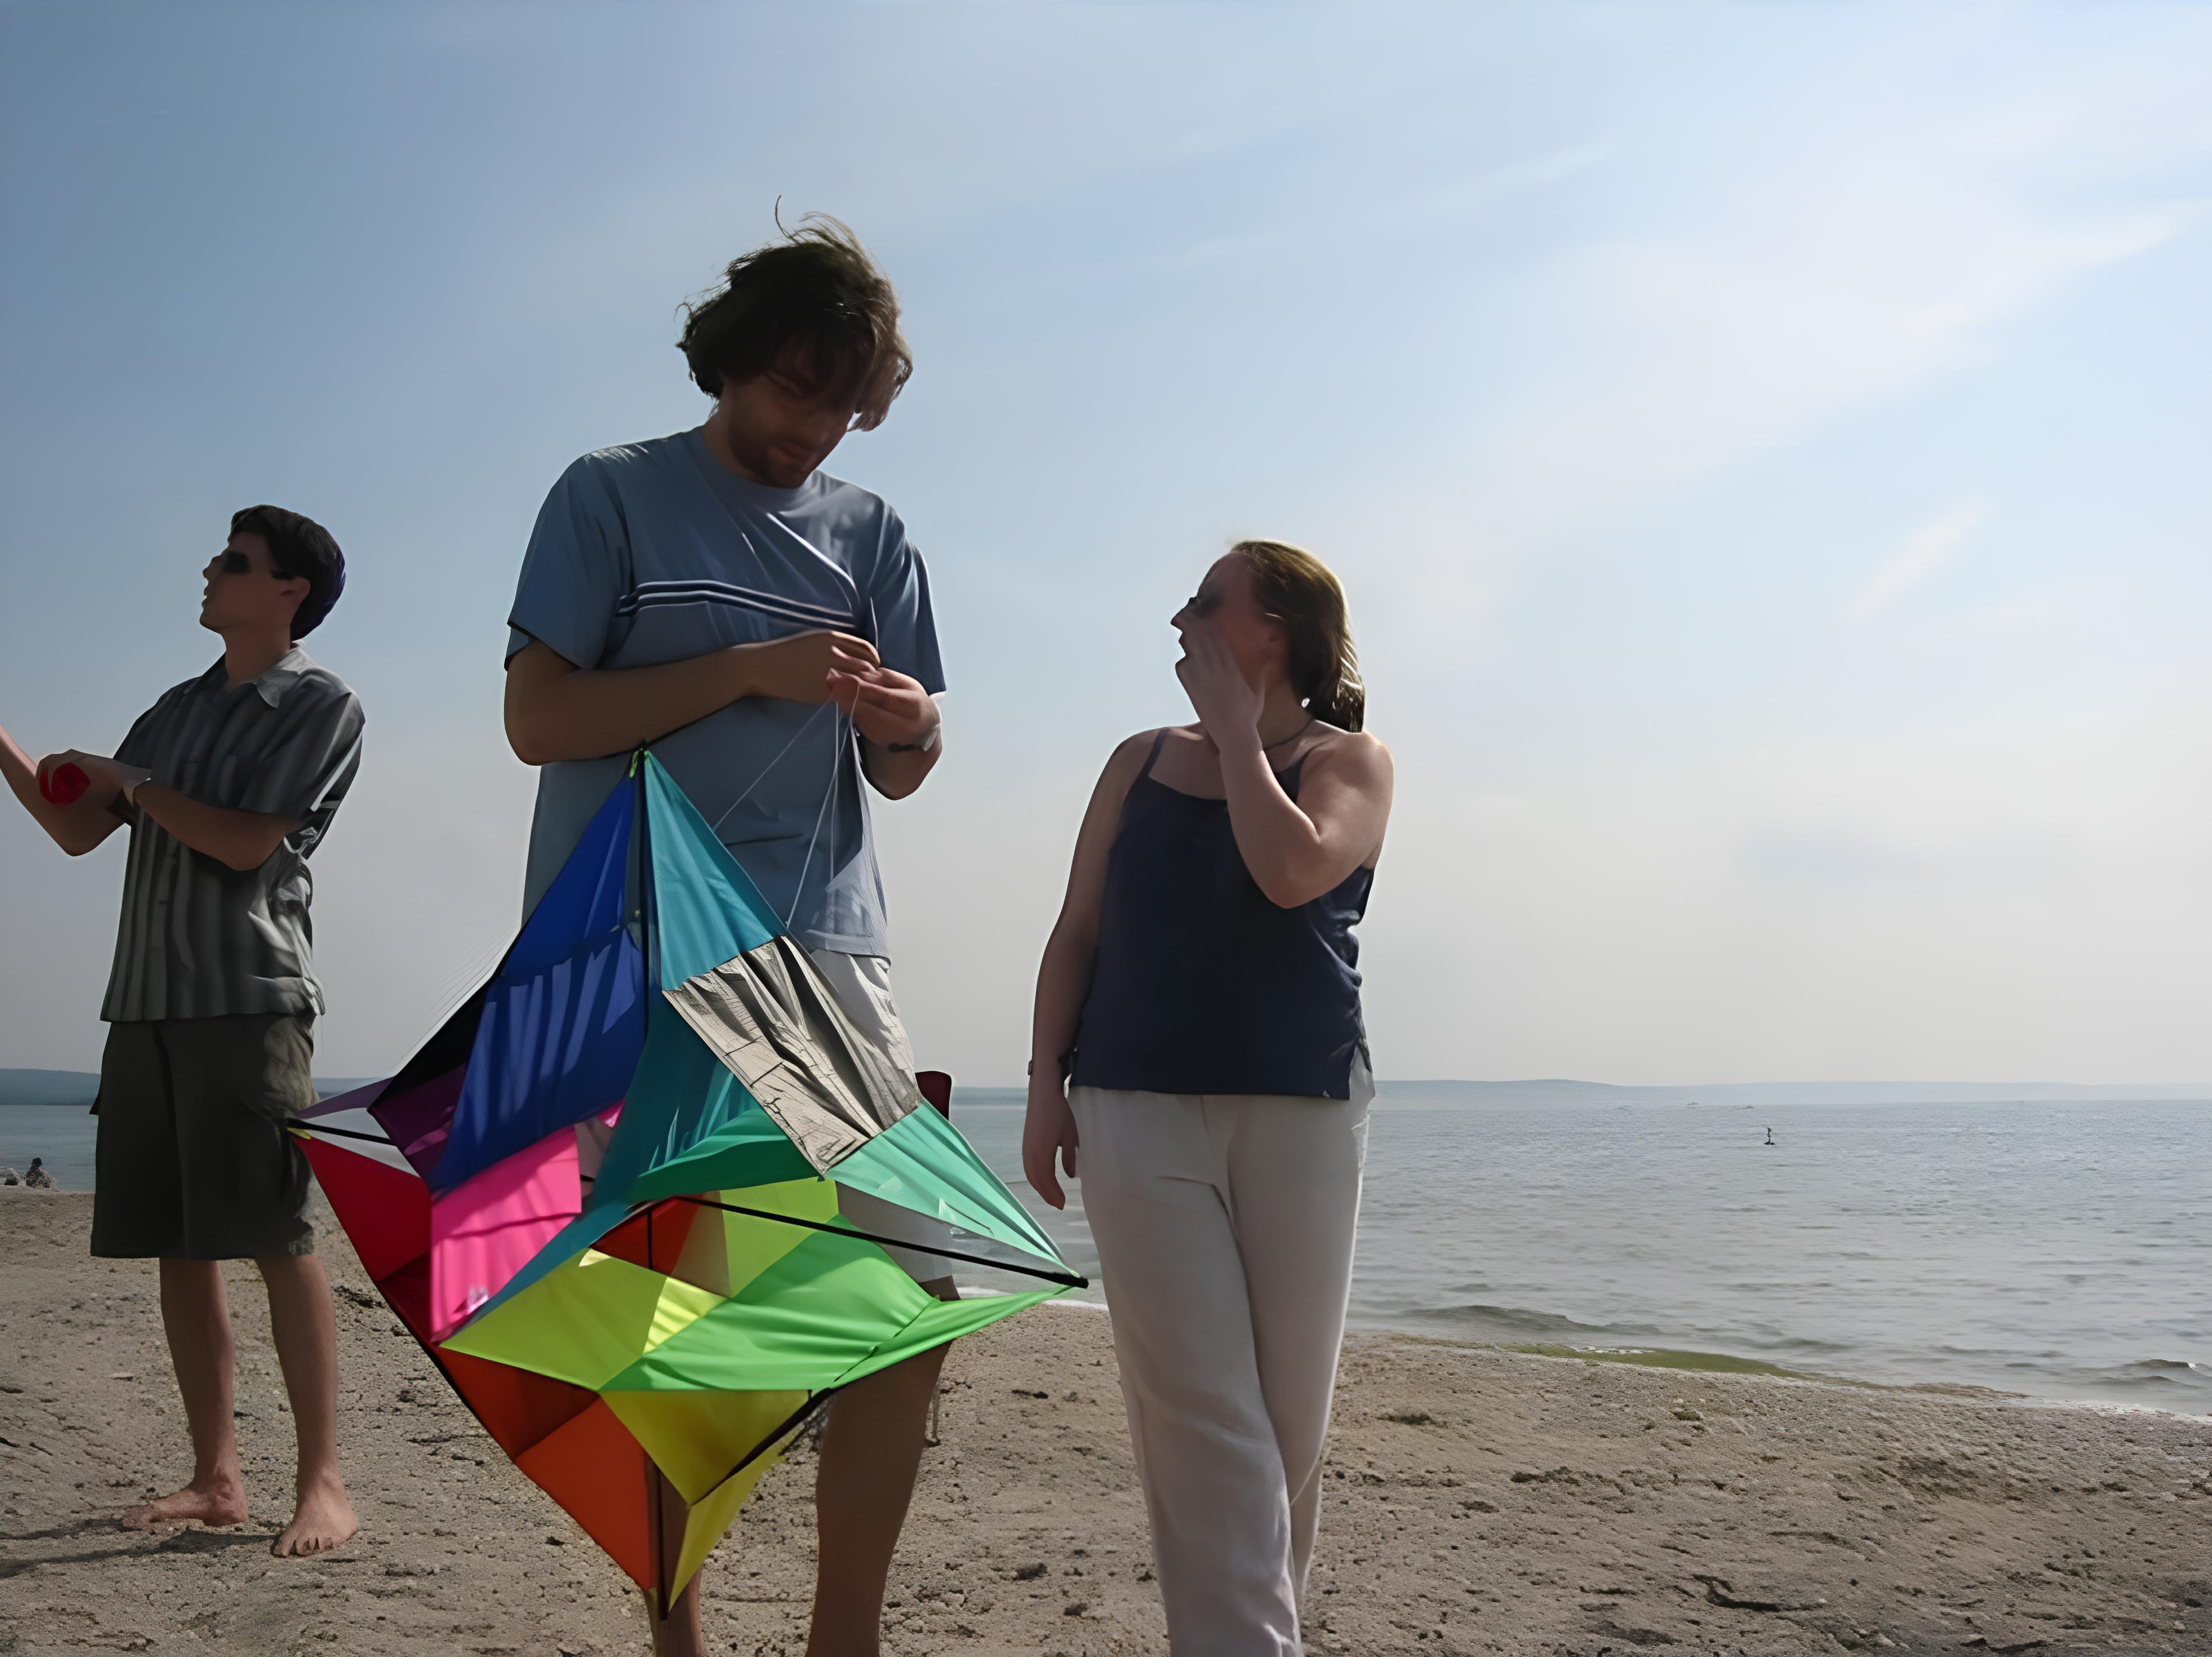
\includegraphics[width=0.23\textwidth]{images/original-segmentation.png}}
	\hspace{0.01\textwidth}
	\subfloat[]{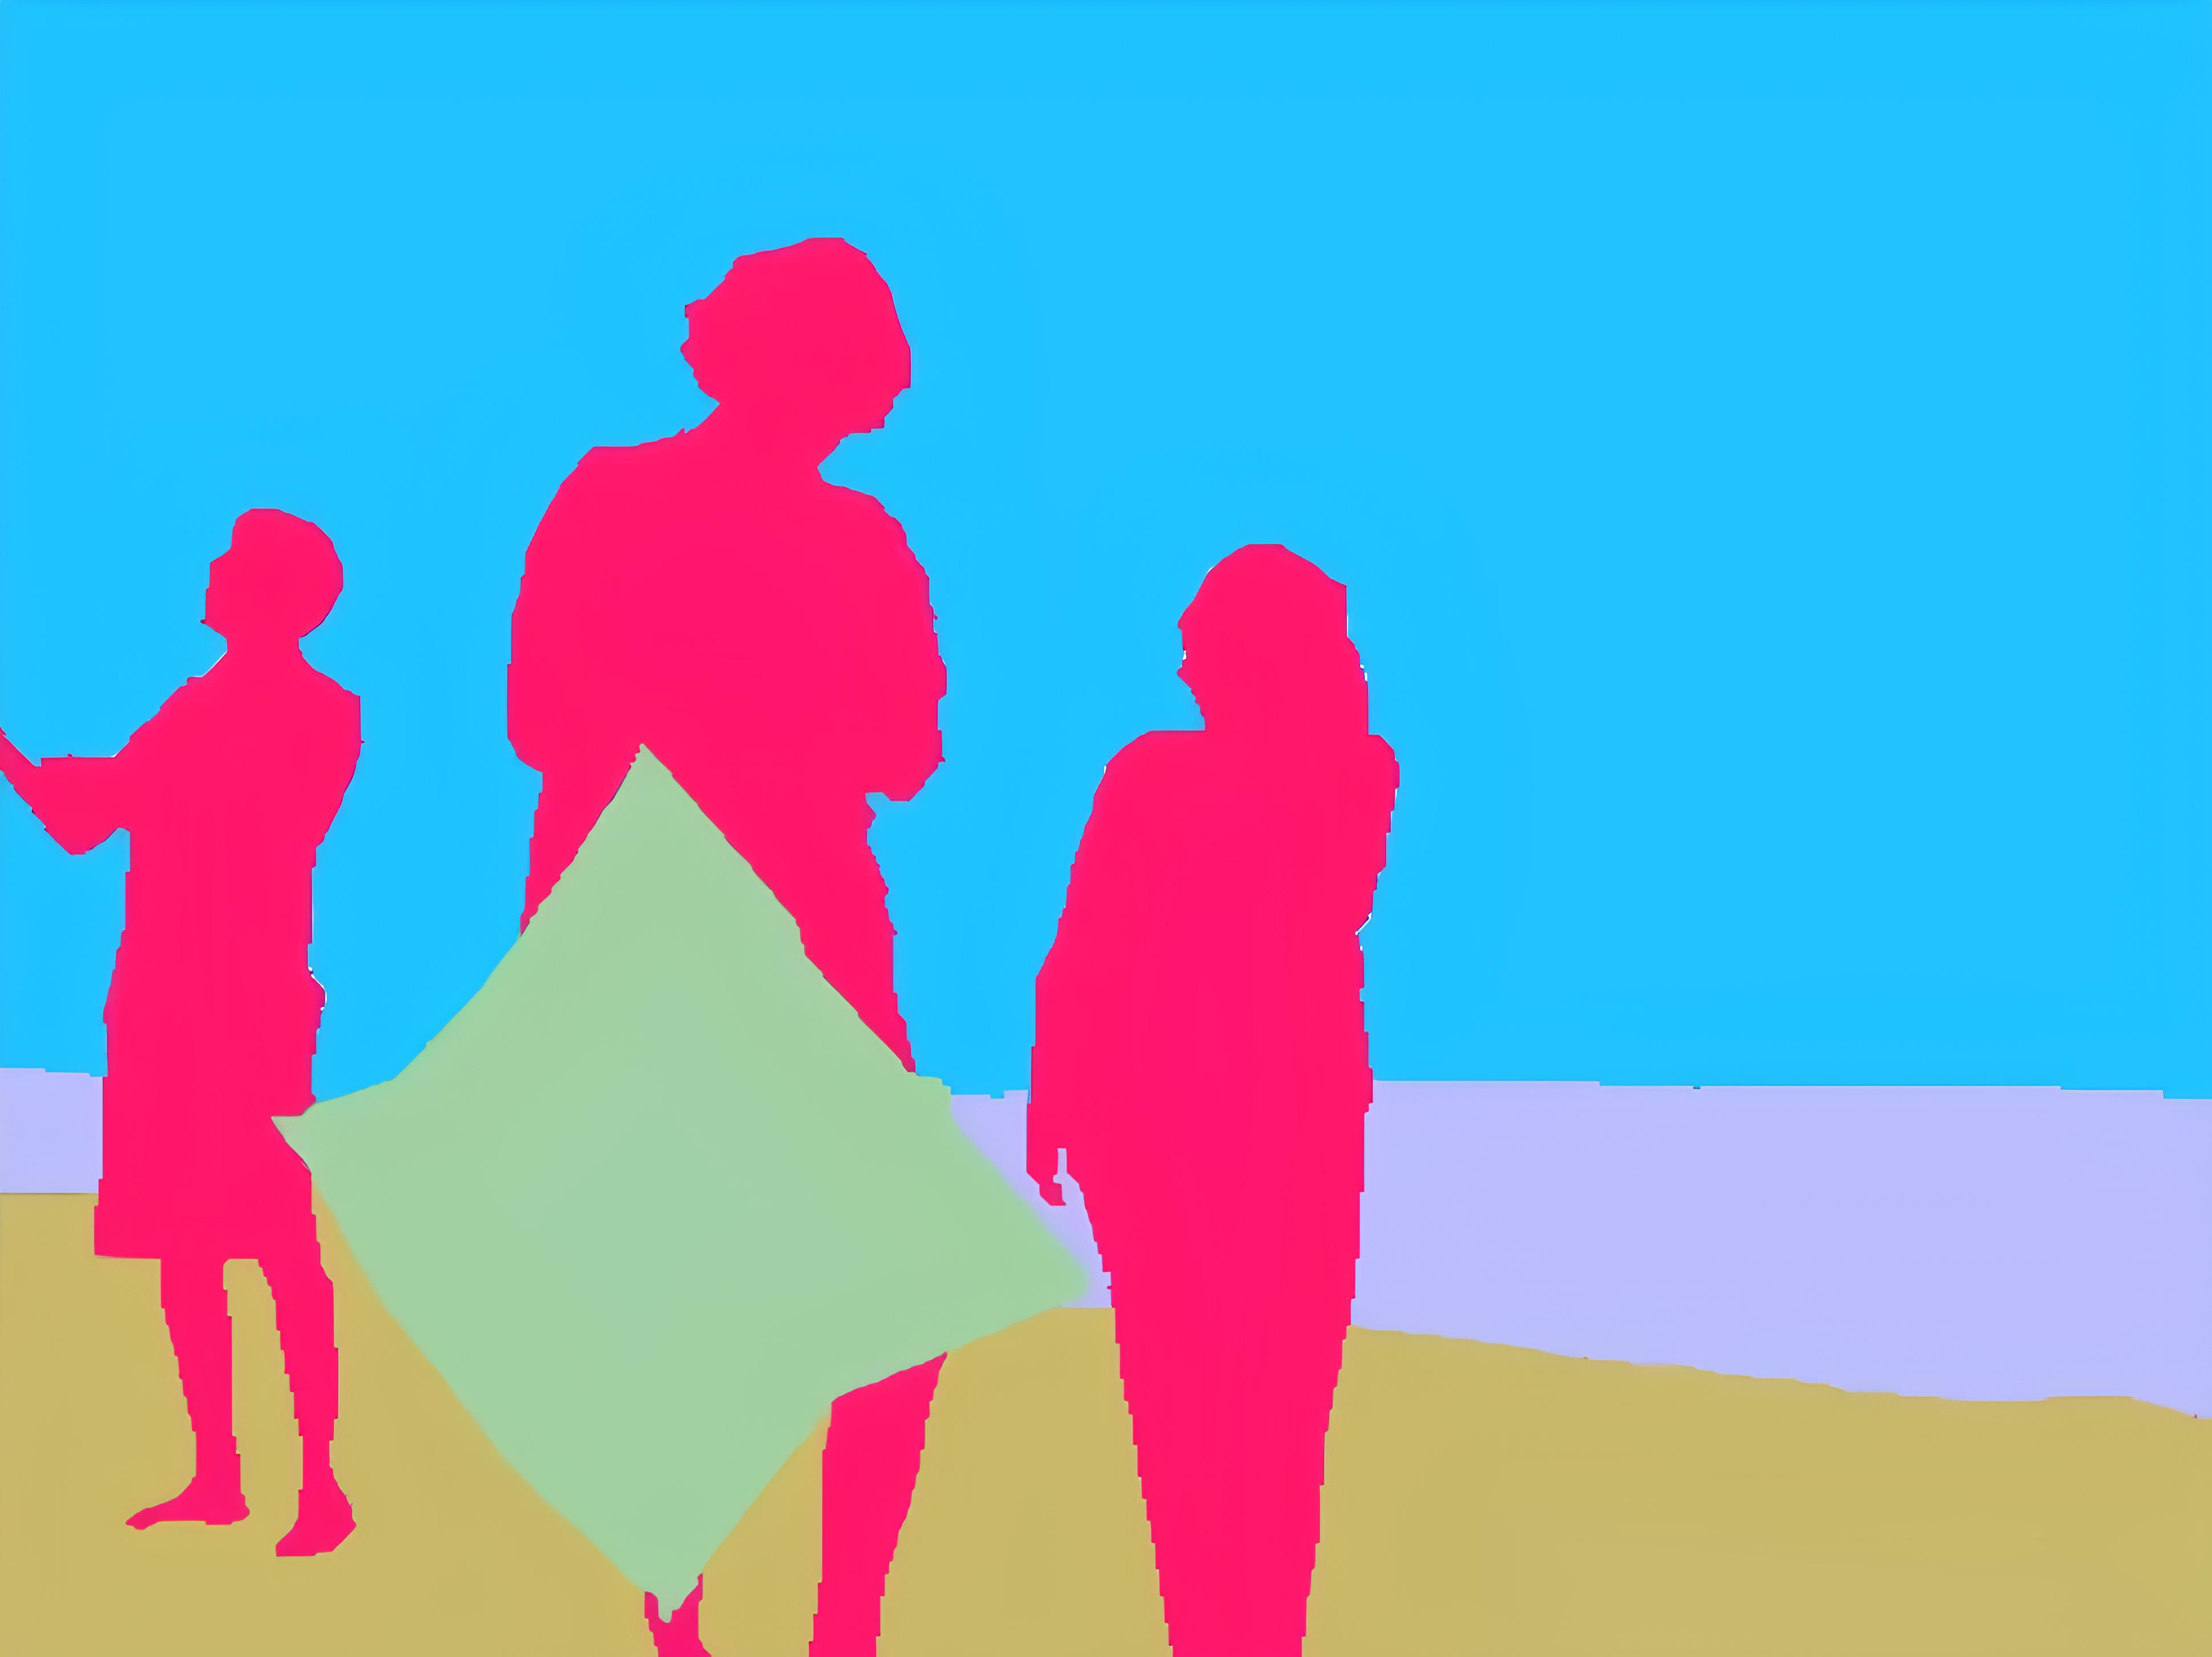
\includegraphics[width=0.23\textwidth]{images/semantic-segmentation.png}}
	\hspace{0.01\textwidth}
	\subfloat[]{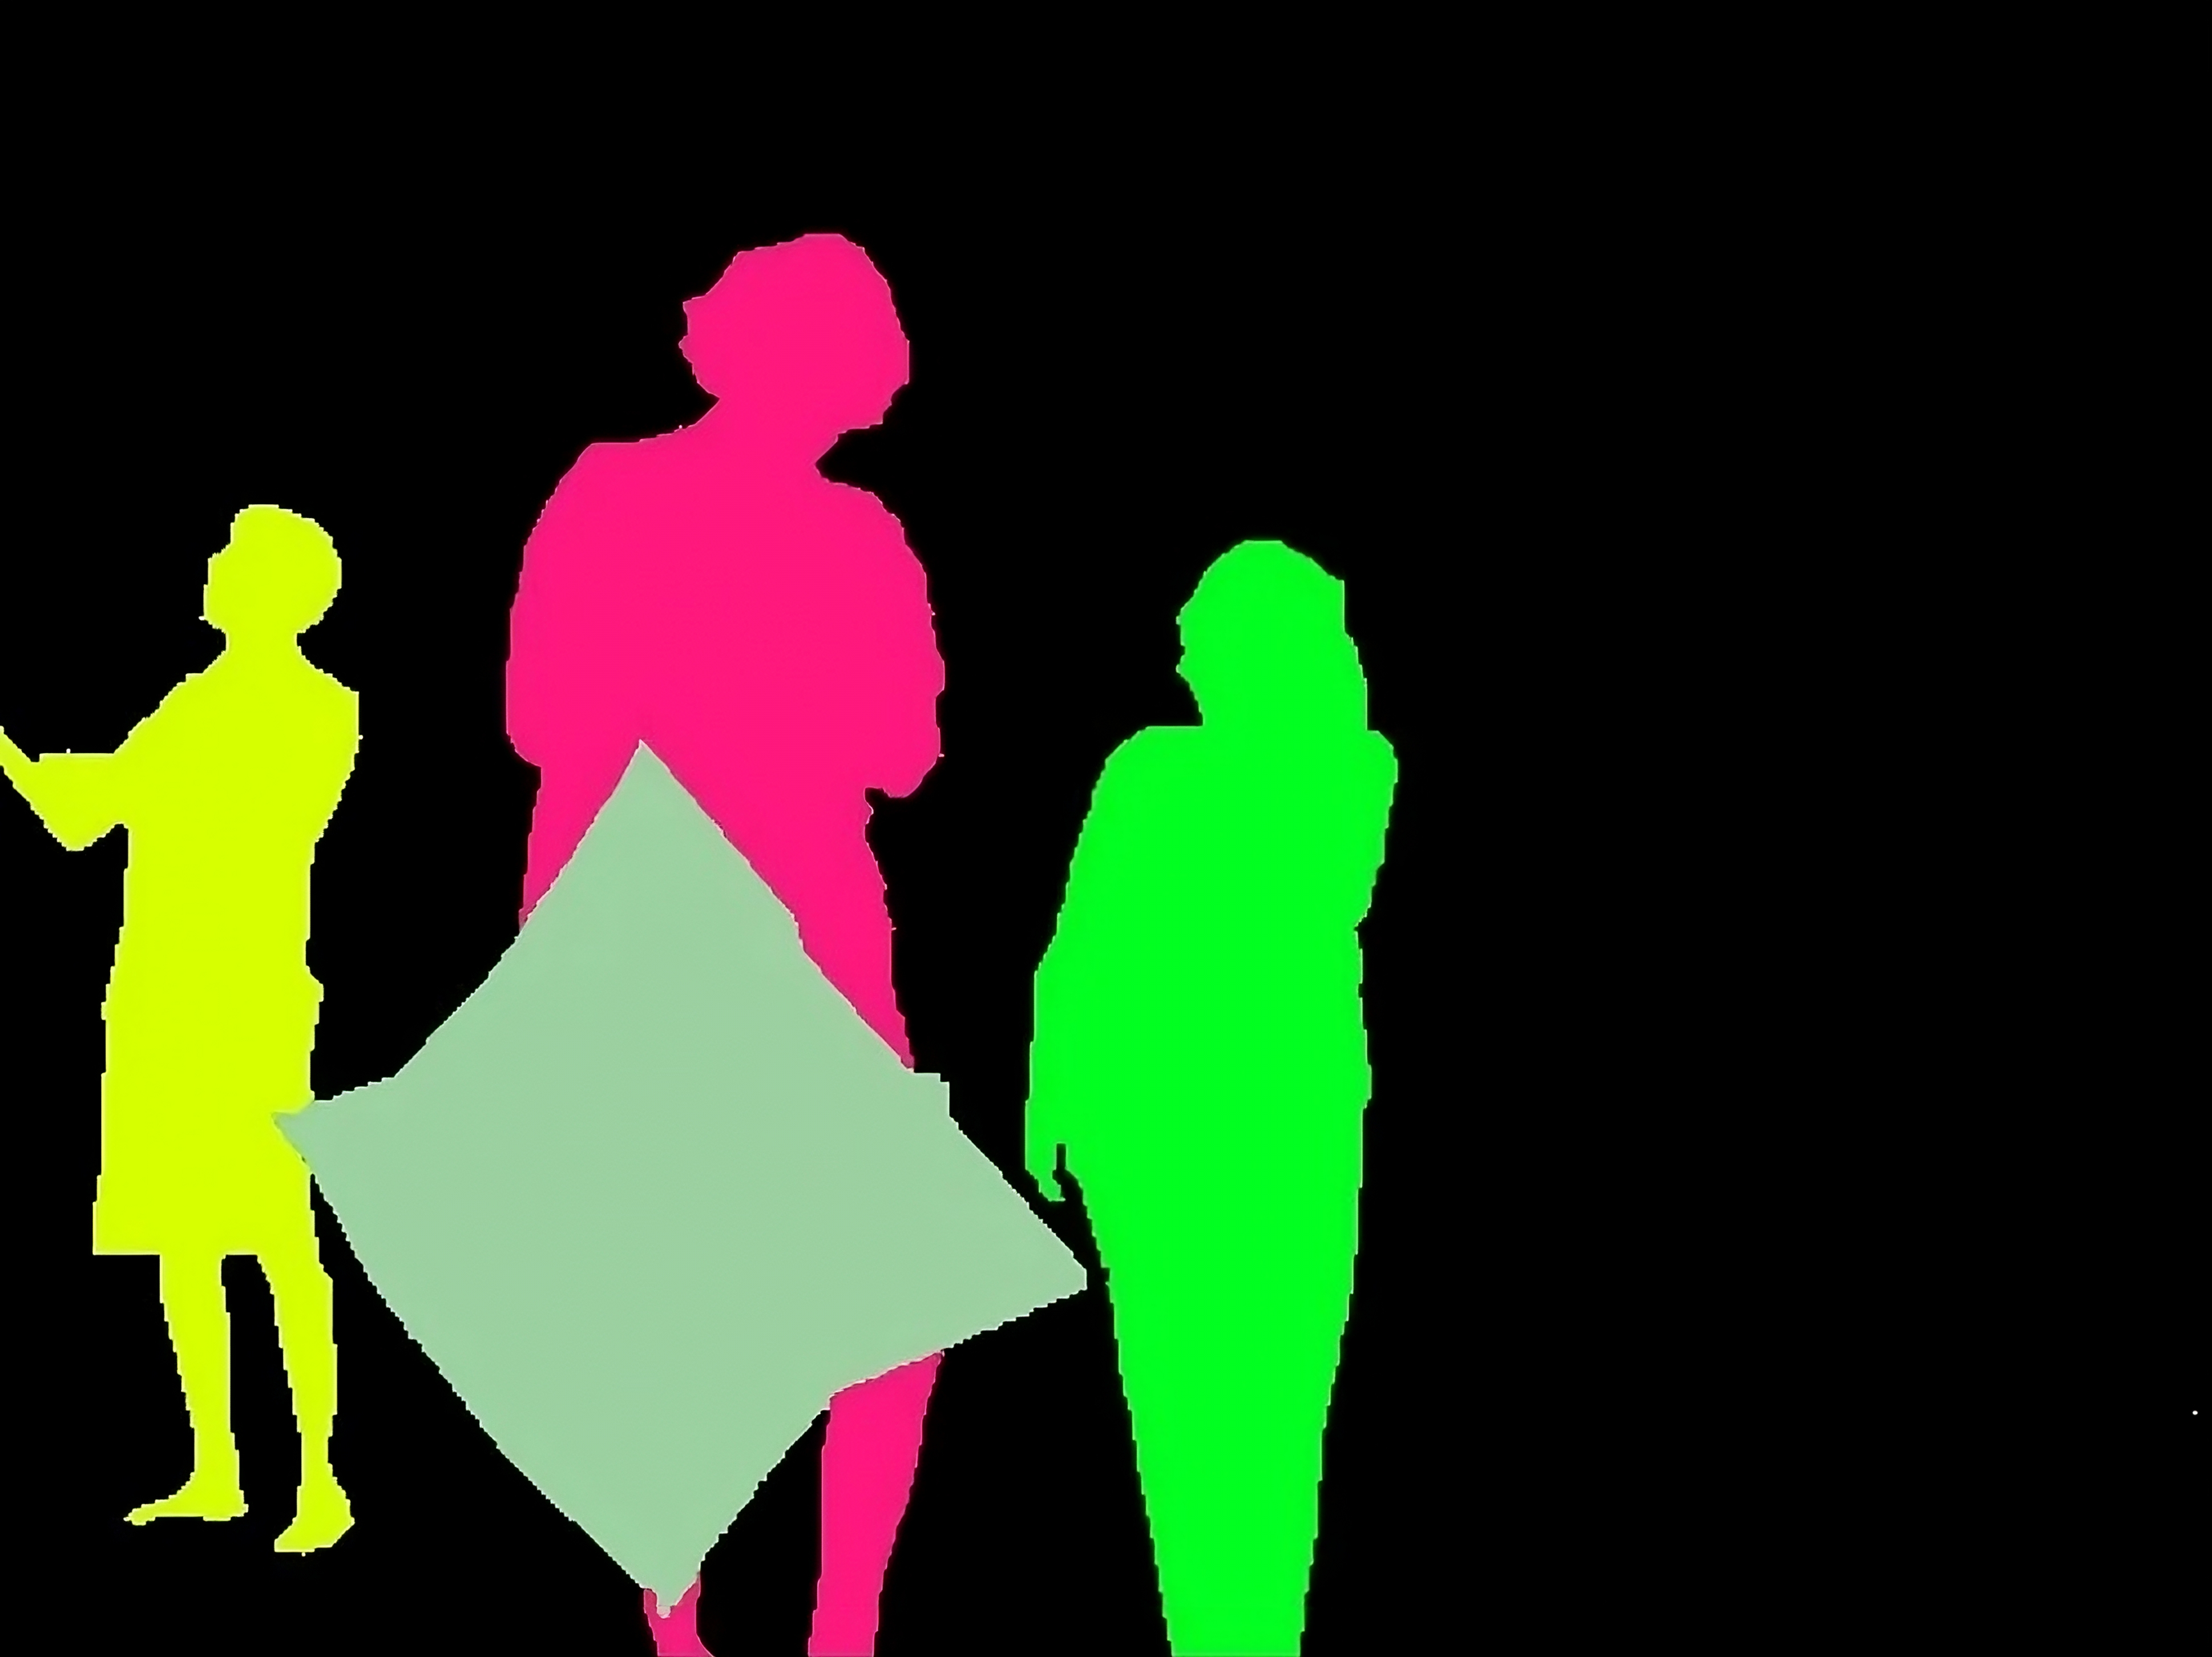
\includegraphics[width=0.23\textwidth]{images/instance-segmentation.png}}
	\caption{Data un'immagine (a), esempio di segmentazione semantica (b) e segmentazione d'istanza (c).}
	\label{fig:segmentazione}
\end{figure}

Il nostro approccio si basa su due componenti principali: un modello di segmentazione semantica (\textit{segmentatore}) addestrato con dati simulati, che opera in modo ottimale solo con dati provenienti dal simulatore stesso, e un sistema di trasformazione dei dati reali.

Bisogna quindi trasformare i dati reali in dati simili a quelli simulati, proiettando le immagini reali sul dominio della simulazione. Questa trasformazione viene effettuata tramite una seconda rete neurale profonda con architettura encoder-decoder. Il compito di questo secondo modello è quello di rielaborare i dati reali ricevuti in ingresso, e modificarli in modo da farli corrispondere alle caratteristiche attese dal segmentatore. L'output dell'encoder-decoder viene quindi utilizzato come input del segmentatore, che a questo punto riuscirà a fare correttamente inferenza sul dato ricevuto.

Il modo più semplice e intuitivo per addestrare l'encoder-decoder consiste nel prendere il segmentatore pre-addestrato sui dati simulati e congelare i suoi pesi. A questo punto l'encoder-decoder viene co-addestrato utilizzando la funzione di loss calcolata dal segmentatore. Durante il processo di addestramento i dati attraversano prima l'encoder-decoder, il suo output diventa l'input del segmentatore che a sua volta calcola la loss. A questo punto si effettua la backpropagation, che aggiorna solo i pesi dell'encoder-decoder e che lascia invariati quelli del segmentatore.

Una criticità di questo approccio è la necessità di disporre di una piccola quantità di dati reali segmentati per l'addestramento dell'encoder-decoder. Questa limitazione, nonostante rappresenta un potenziale sventaggio, è significativamente meno onerosa rispetto a realizzare grandi dataset annotati richiesti da altre tecniche. Uno schema riassuntivo dell'architettura proposta è illustrato nella \hyperref[fig:architettura-unet-yolo]{Figura \ref{fig:architettura-unet-yolo}}.

\begin{figure}[t]
	\centering
	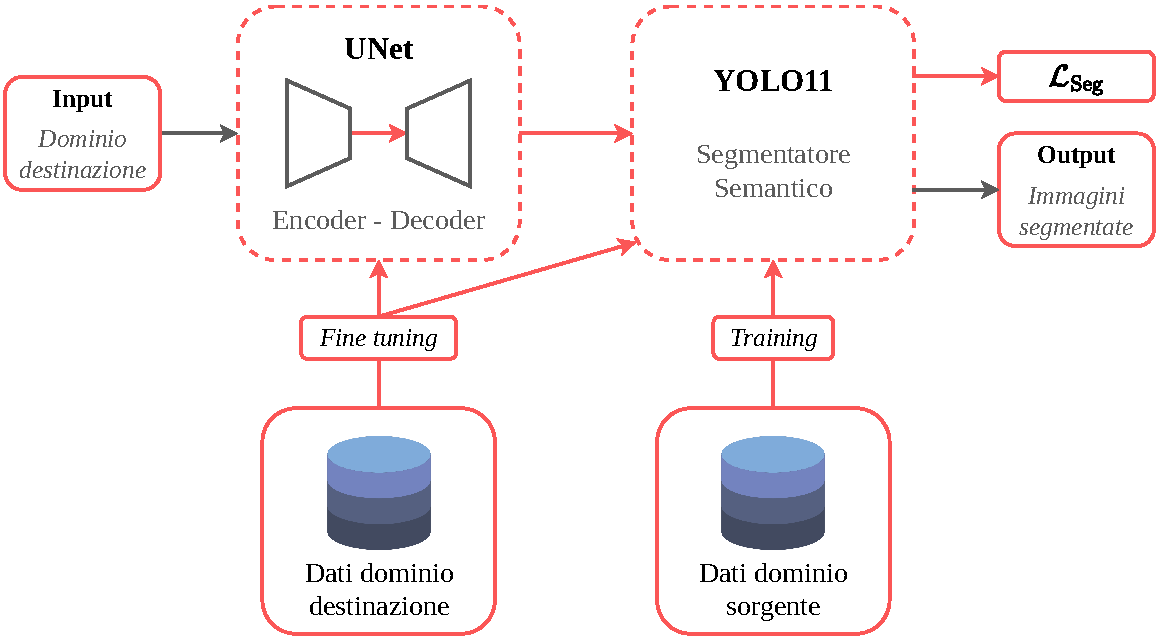
\includegraphics[width = \textwidth, clip]{images/unet-yolo-architecture}
	\caption{Schema dell'architettura real-to-sim}
	\label{fig:architettura-unet-yolo}
\end{figure}

\section{Strumenti}
\label{chap:strumenti}

In questa sezione verranno descritti i diversi strumenti utilizzati in questo elaborato per implementare l'architettura proposta. La scelta di ciascuno strumento è stata guidata da considerazioni relative alle esigenze del progetto e alle caratteristiche tecniche necessarie.

\subsection{Simulatore}
\label{chap:simulatore}

Questo elaborato si basa in parte sul lavoro pregresso realizzato da Riccardo Raffini, che nell'A.A. 2022/2023 ha posto le fondamenta per questa tesi. Raffini ha realizzato un'architettura capace di campionare automaticamente dati da un ambiente simulato, fornendo risultati che hanno guidato la scelta degli strumenti utilizzati in questo progetto. Si può quindi dire che la seguente tesi è un continuo della sua ricerca.

Il simulatore scelto da Raffini è stato iGibson 2.0~\cite{li2021igibson}. A differenza di altre soluzioni, iGibson consente di eseguire un insieme generico di attività domestiche. Questo elemento è fondamentale se l'obiettivo finale è generare e raccogliere campioni di dati relativi ad attività robotiche, non solo inerenti alla navigazione o esplorazione dell'ambiente. In questo simulatore, gli oggetti sono caratterizzati da uno stato (temperatura, umidità, pulizia) che non è definito da semplici valori booleani (caldo/freddo, asciutto/bagnato, pulito/sporco), ma da uno stato fisico esteso. Si cerca quindi di riprodurre in maniera fedele i fenomeni fisici che stanno alla base dei cambiamenti di stato, aumentando così il livello di dettaglio raggiungibile dalle varie attività. Altra peculiarità importante del simulatore, è l'integrazione di un sistema generativo basato su predicati logici. Questo permette di creare scene densamente popolate di oggetti provenienti dai vari dataset~\cite{doi:10.1177/0278364919844314}~\cite{pmlr-v164-srivastava22a}. Questo simulatore si differenzia dagli altri anche per l'integrazione di un'interfaccia di realtà virtuale, funzione che può risultare utile per alcune finalità di ricerca.

Di base iGibson include 15 diverse scene. Ogni scena è semanticamente annotata e contiene diverse categorie di oggetti interattivi, così da garantire un'ottima diversificazione per la campionatura dei dati. Inoltre, il simulatore consente di rendere casuale texture e mesh di ogni singolo oggetto, e in aggiunta permette di caricare scansioni di ambienti reali.

\subsection{Dataset simulato}
\label{chap:dataset_simulato}

Per il suo elaborato, Raffini ha sviluppato un pacchetto ROS~\cite{quigley2009ros} (Robot Operating System) che, integrato al simulatore, permette di controllare un robot di servizio all'interno di un ambiente simulato. Grazie all'architettura progettata, questo robot è in grado di muoversi autonomamente nell'ambiente e raccogliere dati, successivamente elaborati e salvati in un dataset tramite un apposito modulo. Complessivamente sono stati raccolti 60 dataset, campionati da 15 diverse scene.

Questi dataset sono stati concepiti principalmente per addestrare modelli capaci di rilevare oggetti, in particolare per individuare porte e classificare il loro stato (aperte/chiuse). Tuttavia, le immagini raccolte si prestano anche per scopi più generici, come nel nostro caso. I dati sono stati campionati con una frequenza pari a \SI{1}{\hertz}, e ogni campionatura comprende quattro tipologie di immagini: un'immagine RGB dell'ambiente, una mappa di profondità, un'immagine per la segmentazione semantica e una per la segmentazione d'istanza. Sono inoltre presenti dati relativi alle bounding box delle porte, la posa del robot nell'istante della rilevazione, e la posa finale di goal.

\subsection{Segmentatore Semantico}
\label{chap:segmentatore_semantico}

La scelta del segmentatore semantico è stata una delle decisioni più importanti dell'intero progetto, in quanto tutto il lavoro successivo si sarebbe basato interamente su questo modello. Cambiarlo in corsa avrebbe voluto dire rincominciare tutto da capo. Quelli inizialmente considerati per questo lavoro sono stati YOLO11, DETR e Detectron2.

\subsubsection{YOLO11}

YOLO~\cite{JIANG20221066}, acronimo di \textit{You Only Look Once}, è un algotritmo ampiamente utilizzato~\cite{sultana2020review} per la rilevazione e classificazione di oggetti. I suoi principali punti di forza risiedono nelle piccole dimensioni del modello e nel breve tempo necessario per l'inferenza. La sua struttura è semplice e diretta; è infatti in grado di predire posizioni e categorie di oggetti tramite reti neurali, e il tutto in una singola scansione dell'immagine. Questo lo rende molto veloce e adatto ad analizzare flussi video in tempo reale. YOLO possiede inoltre una forte capacità di generalizzazione, consentendogli di apprendere caratteristiche da trasferire ad altri ambienti.

L'architettura YOLO si basa su tre componenti fondamentali. La \textit{backbone}, estrae caratteristiche utilizzando reti neurali convoluzionali, trasformando i dati grezzi delle immagini in mappe di caratteristiche multi-scala. Il \textit{neck} agisce come uno stadio intermedio di elaborazione, e permette di aggregare e migliorare le rappresentazioni delle caratteristiche attraverso diverse scale. Infine, la \textit{head}, genera gli output finali localizzando e classificando gli oggetti secondo le mappe precedentemente elaborate.

Sulla base di quest'architettura, YOLO11 estende e migliora quanto realizzato dai suoi predecessori, introducendo nuove migliorie architetturali e ottimizzando al contempo i parametri. Rispetto a YOLOv8, YOLO11 ha una mAP (\textit{mean Average Precision}) più elevata sul dataset COCO, riducendo allo stesso tempo il numero di parametri del 22\%~\cite{khanam2024yolov11overviewkeyarchitectural}. Sono state inoltre raggiunte velocità di elaborazione più elevate, ed è stato migliorato il processo di estrazione delle caratteristiche della backbone e del neck. YOLO11 è stato progettato per essere utilizzato efficacemente sia su piattaforme cloud, che tu dispositivi edge, aumentando così il numero di casi d'uso.

\subsubsection{DETR}

Il modello \textit{DEtection TRansformers}, abbreviato DETR~\cite{carion2020end}, è stato un notevole passo in avanti nell'ambito della rilevazione di oggetti. Questo approccio, ideato dai ricercatori di Facebook, unisce infatti i benefici delle reti neurali profonde a quelli dei transformer~\cite{10.1145/3505244}, portando ad un'architettura più semplice e con predizioni più accurate anche in caso di sovrapposizione di oggetti. Inoltre, l'utilizzo dei transformer consente di catturare in modo ottimale le relazioni tra gli oggetti e il contesto globale dell'immagine.

L'architettura si compone di una rete neurale convoluzionale e di un transformer, seguito da una serie di reti neurali dirette~\cite{article_890416} (FNN, Forward Neural Network). I transformer sono stati inizialmente ideati nell'ambito dell'elaborazione del linguaggio naturale (NLP, Natural Language Processing), e DETR è innovativo in quanto primo modello di computer vision ad integrare questo componente.

Questo modello risulta innovativo sotto molti punti di vista, presenta anche diverse sfide e limitazioni. Addestrare DETR può risultare infatti costoso in termini di risorse hardware e tempo richiesto, in particolare a causa della presenza dei transformer. In aggiunta, l'addestramento richiede dataset di grandi dimensioni, il che ne limita l'uso in contesti in cui i dati disponibili sono limitati.

\subsubsection{Detectron2}

Detectron2 è un altro modello sviluppato dal gruppo di ricerca di Facebook. Questo modello offre performance eccellenti per compiti di segmentazione semantica su immagini singole, ma richiede hardware costoso sia per l'addestramento che per l'inferenza. Queste limitazioni rendono difficile poter lavorare su flussi di dati in tempo reale, e le sue numerose dipendenze risultano un problema per rilasciarlo in produzione.

La scelta finale è ricaduta infine su YOLO11, in quando perfetto per l'analisi di flussi video in tempo reale e richiedendo al contempo un numero esiguo di risorse. Questo modello è inoltre presente in cinque formati, ognuno caratterizzato da un numero crescente di parametri e con un conseguente aumento di complessità e di prestazioni. Nella \hyperref[tab:yolo-prestazioni-segmentazione]{Tabella \ref{tab:yolo-prestazioni-segmentazione}} sono riportati i diversi modelli disponibili per YOLO11.

\begin{table}[t]
	\centering
	\begin{tabular}{
			@{}l
			>{\centering\arraybackslash}p{2cm}
			>{\centering\arraybackslash}p{2cm}
			>{\centering\arraybackslash}p{2cm}
			>{\centering\arraybackslash}p{2cm}
			>{\centering\arraybackslash}p{2cm}@{}}
		\toprule
		\textbf{Modello} & 
		\begin{tabular}[c]{@{}c@{}}\textbf{Immagine}\\ \footnotesize{(pixel)}\end{tabular} & 
		$\textbf{mAP}^{\text{box}}_{50-95}$ & 
		$\textbf{mAP}^{\text{mask}}_{50-95}$ & 
		\begin{tabular}[c]{@{}c@{}}\textbf{Velocità} \\ NVIDIA T4 \\ \footnotesize{(ms)}\end{tabular} & 
		\begin{tabular}[c]{@{}c@{}}\textbf{Parametri} \\ \footnotesize{(M)}\end{tabular} \\
		\midrule
		YOLO11n-seg & 640 & 38.9 & 32.0 & $1.8 \pm 0.0$ & 2.9 \\
		\rowcolor[HTML]{F4F4F4} YOLO11s-seg & 640 & 46.6 & 37.8 & $2.9 \pm 0.0$ & 10.1 \\
		YOLO11m-seg & 640 & 51.5 & 41.5 & $6.3 \pm 0.1$ & 22.4 \\
		\rowcolor[HTML]{F4F4F4} YOLO11l-seg & 640 & 53.4 & 42.9 & $7.8 \pm 0.2$ & 27.6 \\
		YOLO11x-seg & 640 & 54.7 & 43.8 & $15.8 \pm 0.7$ & 62.1 \\
		\bottomrule
	\end{tabular}
	\caption{Performance dei vari modelli YOLO11 per la segmentazione semantica.}
	\label{tab:yolo-prestazioni-segmentazione}
\end{table}

\subsection{Dataset reale}
\label{chap:dataset_reale}

\subsection{Encoder-Decoder}
\label{chap:encoder_decoder}

% CAPITOLO 4: Metodo
\chapter{Metodo}
\label{chap:metodo}

\section{Raccolta dati su iGibson}
\label{chap:raccolta_dati_igibson}

\section{Trasformazione dataset iGibson in formato YOLO}
\label{chap:dataset_igibson_yolo}

\section{Addestramento del modello YOLO11}
\label{chap:addestramento_yolo}

\section{Trasformazione dataset ScanNet in formato UNet}
\label{chap:dataset_scannet_unet}

\section{Addestramento del modello UNet}
\label{chap:addestramento_unet}

% CAPITOLO 5: Analisi risultati
\chapter{Analisi risultati}
\label{chap:analisi}

\section{Setup sperimentale}
\label{chap:setup}

\section{Procedure}
\label{procedure}

\section{Risultati}
\label{risultati}

% CAPITOLO 6: Conclusioni
\chapter{Conclusioni}
\label{chap:conclusioni}

\section{Discussione dei risultati}
\label{chap:discussione_risultati}

\section{Limiti della soluzione proposta}
\label{chap:limiti}

\section{Prospettive e sviluppi futuri}
\label{chap:prospettive}

% Bibliografia
\beforebibliography
\bibliographystyle{unsrt}
\bibliography{bibliography}

% Pagina di chiusura
\closingpage

\end{document}
